\documentclass{article}
\usepackage{amssymb}
\usepackage[utf8]{inputenc}
\usepackage[english]{babel}
\usepackage{amsthm}
\usepackage{enumitem}
\usepackage{amsmath}
\usepackage{mathrsfs}
\usepackage{hyperref}
\usepackage{graphicx}
\usepackage{placeins}
\usepackage[hypcap]{caption}
\usepackage{subcaption}
\usepackage[margin=.5in]{geometry}
\usepackage[export]{adjustbox}
\usepackage{listings}
\usepackage{alltt}

\graphicspath{{../Figures/}}

\title{Project 3 Writeup}
\date{05/10/2016}
\author{Andrea Bajcsy \and Michelle Cody \and Charles Parker }

\begin{document}
	\maketitle
	
	\begin{enumerate}
	
	\item[\textbf{WU1}] The normalized eigenvalues are shown in Figure \ref{fig:WU1} below. One needs 81 eigenvectors to account for 90\% of the variance and 135 eigenvectors to account for 95\% of the variance.
	
	\begin{figure}[h!]
		\centering
		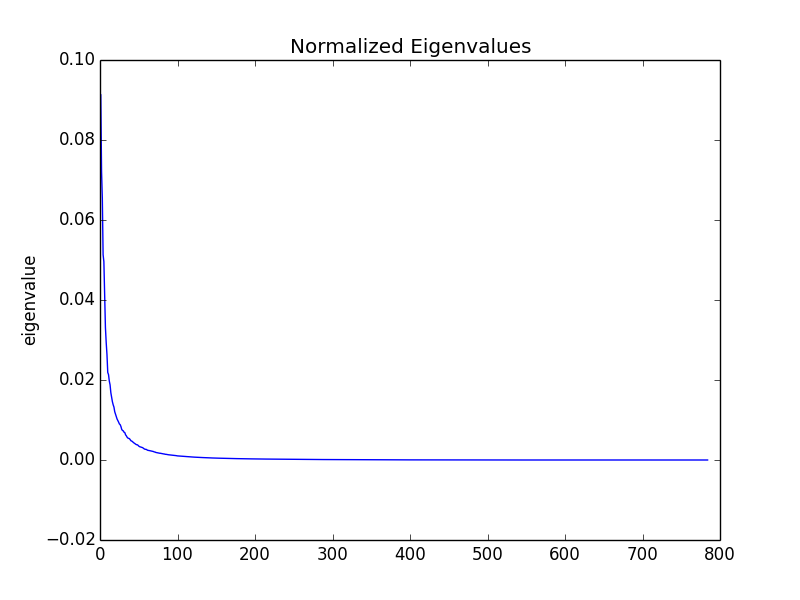
\includegraphics[width=.5\textwidth]{normalized_eigenvalues.png}
		\caption{Normalized eigenvalues of the covariance matrix for the digits data}
		\label{fig:WU1}
	\end{figure}

	\FloatBarrier

	\item[\textbf{WU2}] The plots of the top 50 eigenvectors are shown in Figure \ref{fig:WU2} below. Besides the first few eigenvectors (those corresponding to labels 0 - 5) which very roughly resemble digits, the images do not look like digits. They should not look like digits because the eigenvectors are the directions of most variance. In terms of the image, this corresponds to the weighted combination of pixels at which there is the highest variance. Since all of the digits are represented in the set and some digits share elements of appearance (such as a vertical bar at the center of the image), it would be very unlikely that a direction of large variance would correspond exactly to one particular digit.
	
	\begin{figure}[h!]
		\centering
		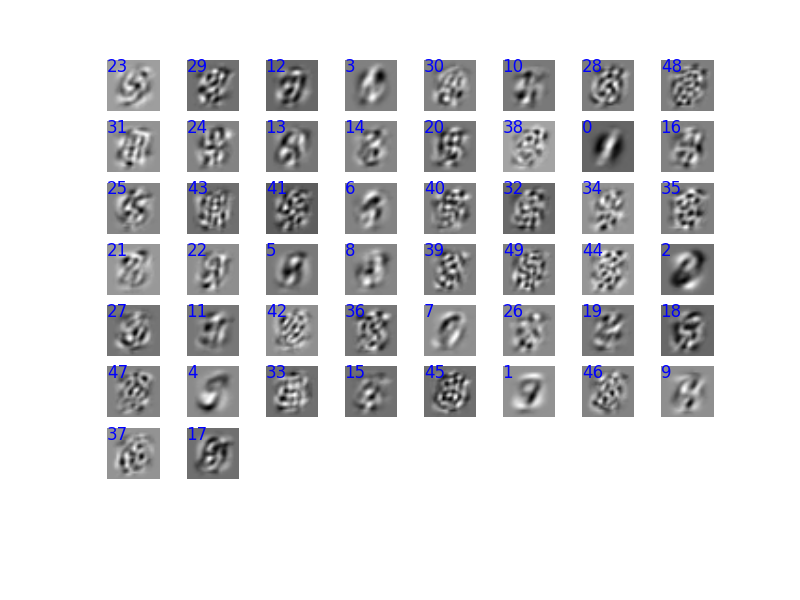
\includegraphics[width=.5\textwidth]{eigvects.png}
		\caption{Top 50 eigenvectors }
		\label{fig:WU2}
	\end{figure}
	
	\FloatBarrier
	
	\item[\textbf{WU3}] 
Yes, you could have fewer support vectors (e.g. 2 vectors). Currently, two of the SV's represent the blue class and one represents the red class (and all of the SV's have the same margin). We could remove one of the SV's of the blue class and still get the same output. 

	\item[\textbf{WU4}]
You get these little blobs because you are summing up the normal distributions around each point. As we turn up gamma, the variance increases and the kernel essentially vanishes. When we up gamma up to 400, we get a little decision boundary around each example (i.e. each decision boundary surrounds exactly one example) (see Figure \ref{fig:WU4}).

\begin{figure}[htp]
\centering
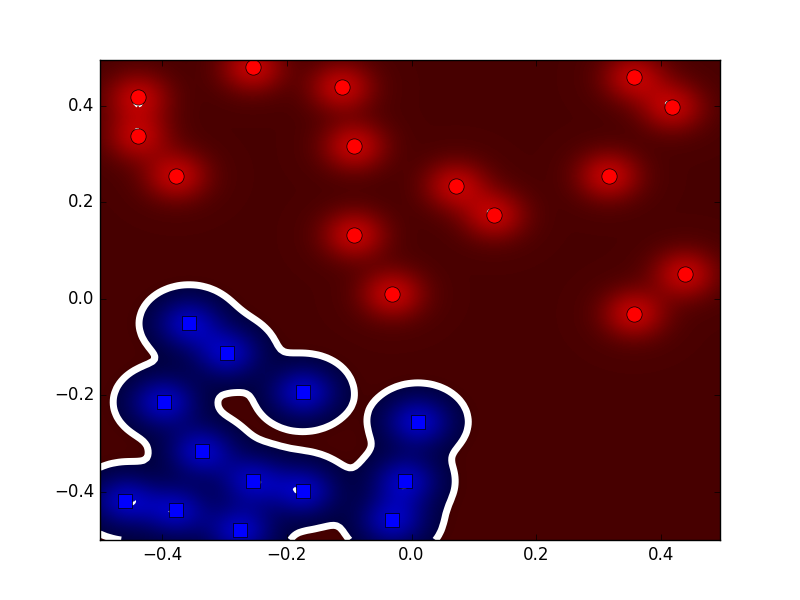
\includegraphics[width=.5\textwidth]{wu4.png}
\caption{SVM with RBF kernel using gamma = 450.}
\label{fig:WU4}
\end{figure}

	\item[\textbf{WU5}]
There are a lot of red support vectors on the blue side of the decision boundary because this data is not linearly separable. 

	\item[\textbf{WU6}]
The 0/1 loss on the training data is not zero because it misclassifies one blue point (in lower right hand corner). The hinge loss on the training data is also not zero because there are many points inside the margin.

	\item[\textbf{WU7}]
When training an RBF kernel on this data, the smallest gamma for which we could get a good decision boundary was gamma = 2. A good decision boundary is defined by a low number of points being used as support vectors and a wider margin (see Figure \ref{fig:WU7}). 

\begin{figure}[htp]
\centering
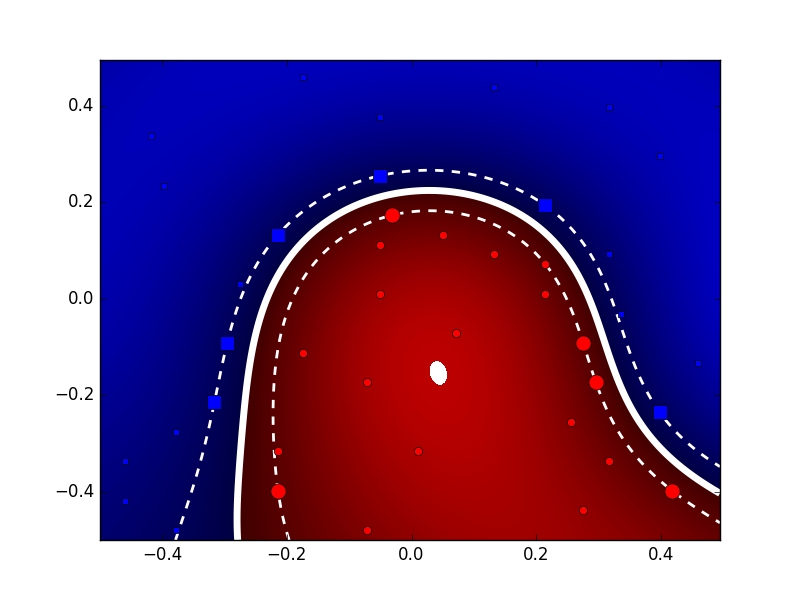
\includegraphics[width=.5\textwidth]{wu7.png}
\caption{Complex dataset with RBF kernel using gamma = 2.}
\label{fig:WU7}
\end{figure}

\pagebreak

\end{enumerate}

\end{document}

